\chapter{Die Skelettierung}
\section{Thinning}
\Autor{Johannes Böhler}\\\\
Das Thinning bezeichnet eine Kategorie von Methoden zur Skelettierung von 2D sowie 3D Objekten. In dieser Projektarbeit ist der Fokus ausschliesslich auf die 2D Skelettierung gerichtet, da die Kinect kein vollkommenes 3D Modell eines Objektes liefert. Sie erfasst das Objekt lediglich aus einem Blickwinkel, desshalb erhält man nur ein 2,5 dimensionales Modell. Es werden nur Tiefeninformationen bezüglich Seite des Objektes, welche der Kinect zugewendet ist bereitgestellt. Die  Tiefeninformationen der Rückseite bleiben verborgen. Um ein vollständiges 3D Modell zu erhalten müssten mindestens 2 Kinects verwendet werden und die Informationen beider Geräte zusammengeführt und vereinheitlicht werden. 

Alle Thinning Algorithmen verbindet das iterative Abtragen des Musters oder der Oberfläche.

\section{Distanztransformation}
%Sandra: Theorie über Skelettierung mit der Distanztransformation
\section{Weitere Verfahren}
\section{Verwandte Arbeiten}
\subsection{Extracting Skeletons From Distance Maps}
%Sandra
\begin{figure}
\centering
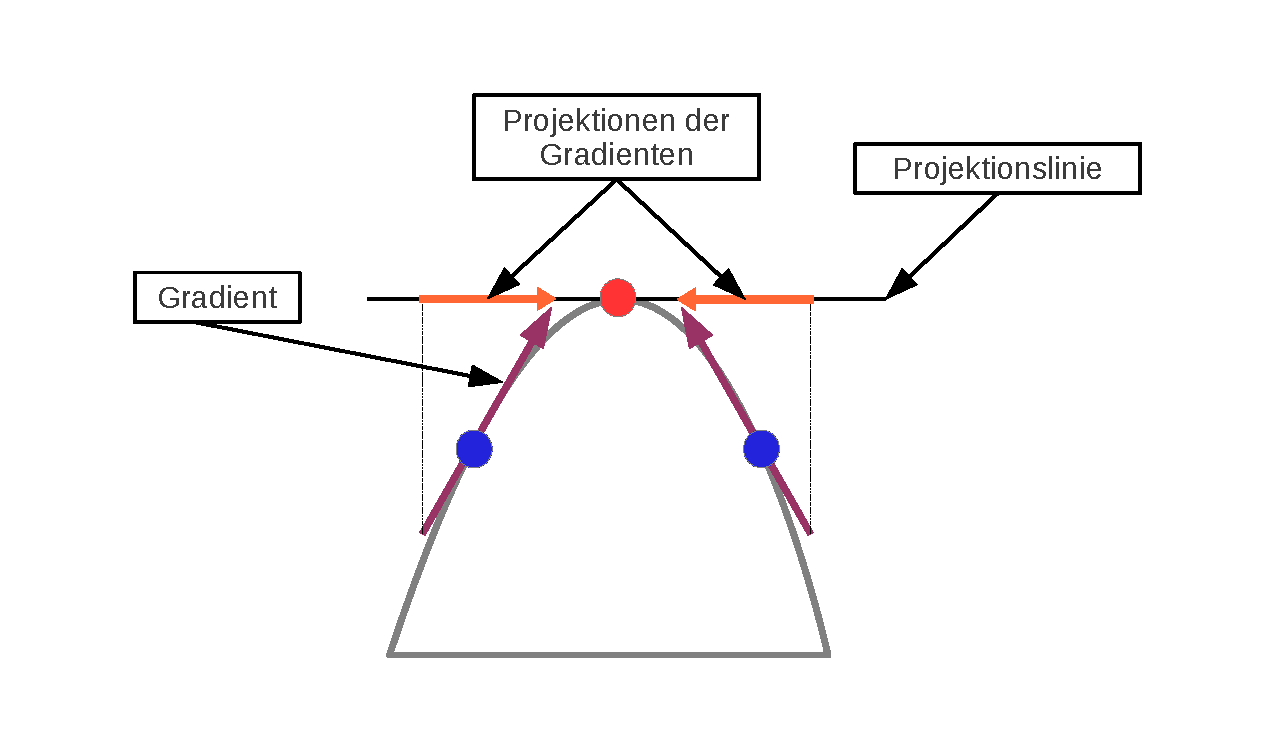
\includegraphics[width=0.6\linewidth]{./fig/paper_ridge_point_detection}
\caption{Ridge Point Detection}
\label{fig:paper_ridge_point_detection}
\end{figure}
\newpage
\subsection{A Fast Parallel Algorithm for Thinning Digital Patterns} 
\Autor{Johannes Böhler}\\\\
Der Algorithmus ist insgesamt in mehrere Iterationen unterteilt. Die Randpixel des Musters werden Schicht für Schicht abgetragen. Die Iterationen sind selbst wiederum in mehrere Subiterationen unterteilt. Das Abtragen der „Schichten“ wird somit in zwei unterschiedliche Phasen aufgespalten
Mit Hilfe der ersten Subiteration werden sowohl Süd- und Ostgrenzpunkte als auch Nordwest Eckpunkte entfernt. \\


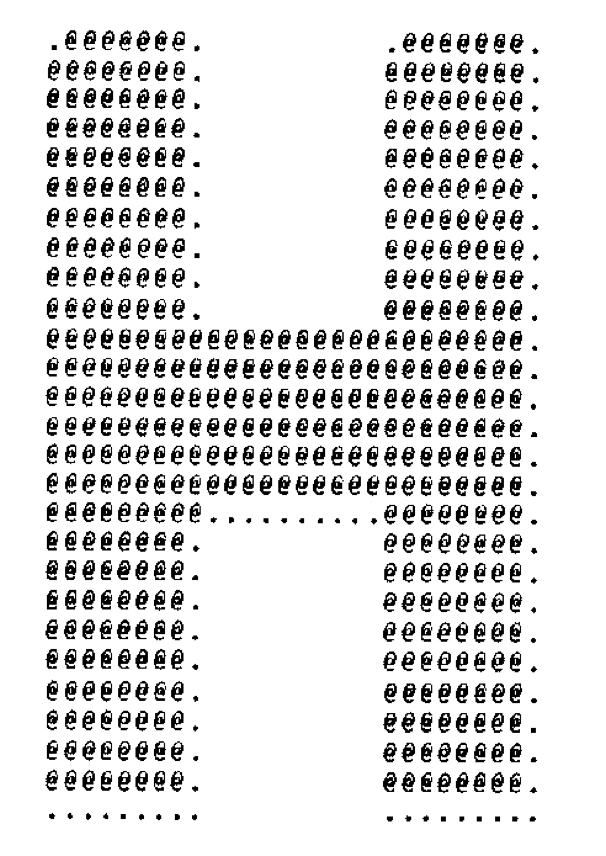
\includegraphics[width=4cm]{Res/SuedOst.png}


Das entfernen von Nord- und Westgrenzpunkten sowie von Südosteckpunkten erfolgt in der zweiten Subiteration.\\

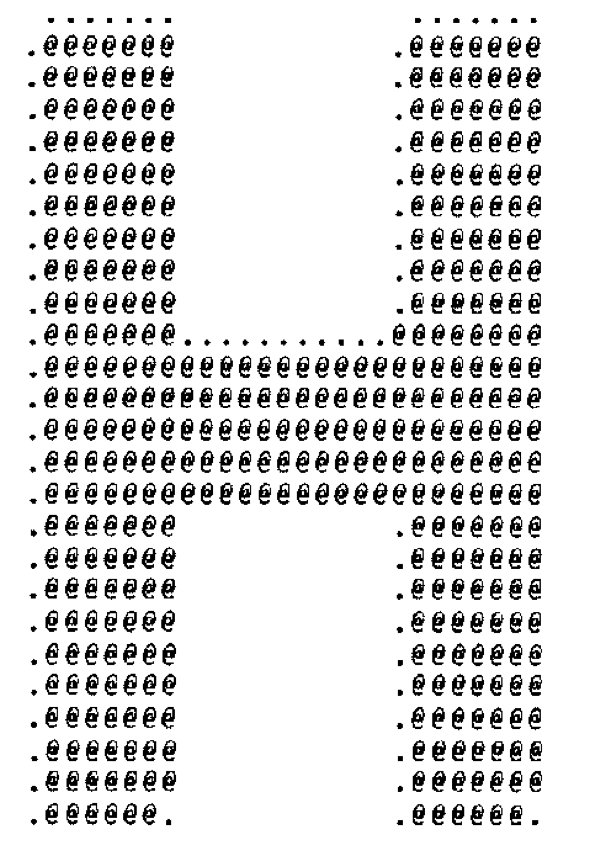
\includegraphics[width=4cm]{Res/NordWest.png}

\subsubsection{Anforderungen an den Algorithmus}

Das Rauschen, welches der Algorithmus verursacht soll so gering wie möglich gehalten werden.
Das Skelett des Ursprungsmusters soll die Endpunkt- und Pixelverbundenheit erhalten.
Endpunktverbundenheit bedeutet, dass sich zwischen zwei Endpunkten eines Skeletts keine unverbundenen Stellen befinden.
Das Skelett soll nach Durchlaufen des kompletten Algorithmus in einheitlicher Dicke von einem Pixel vorliegen.
Der Algorithmus soll möglichst schnell und effizient arbeiten um Echtzeitfähigkeit gewährleisten zu können.\\


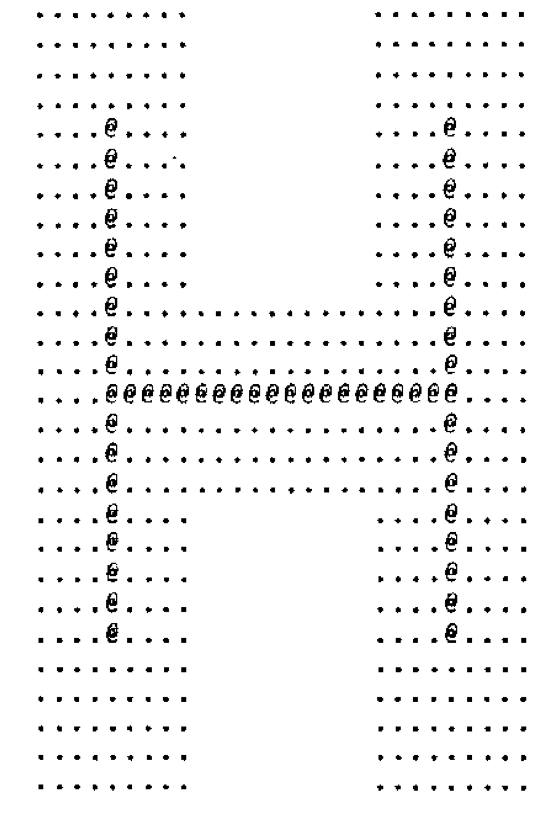
\includegraphics[width=4cm]{Res/Skelett.png}

\subsubsection{Ablauf des Algorithmus}

Es wird davon ausgegangen zu Beginn ein binär digitalisiertes Bild vorliegen zu haben.
Die Pixel werden mit Hilfe einer zweidimensionalen Matrix IT durchlaufen, deren Wert an der jeweiligen Stelle IT(i,j) entweder 0 oder 1 ist.
Mit Muster ist die Menge an Pixeln gemeint, welche den Wert eins haben.
Es werden nun in Abhängigkeit von den 8 Nachbarpixeln, Punkt für Punkt iterative Transformationen auf die Matrix angewendet.

Der neue Wert eines Pixels während der n-ten Iteration hängt von dem eigenen Wert während der (n-1)ten Iteration und den Werten der acht Nachbarn während der (n-1)ten Iteration ab. Dies ermöglicht paralleles Transformieren mehrerer Bildpunkte. 
Die Bedingungen, welche zum Ausführen der Transformation erfüllt sein müssen werden über ein 3x3 Pixel Fenster abgefragt. Der Punkt P1 über dessen Transformation entschieden wird, ist mit allen acht Nachbarn verbunden.\\

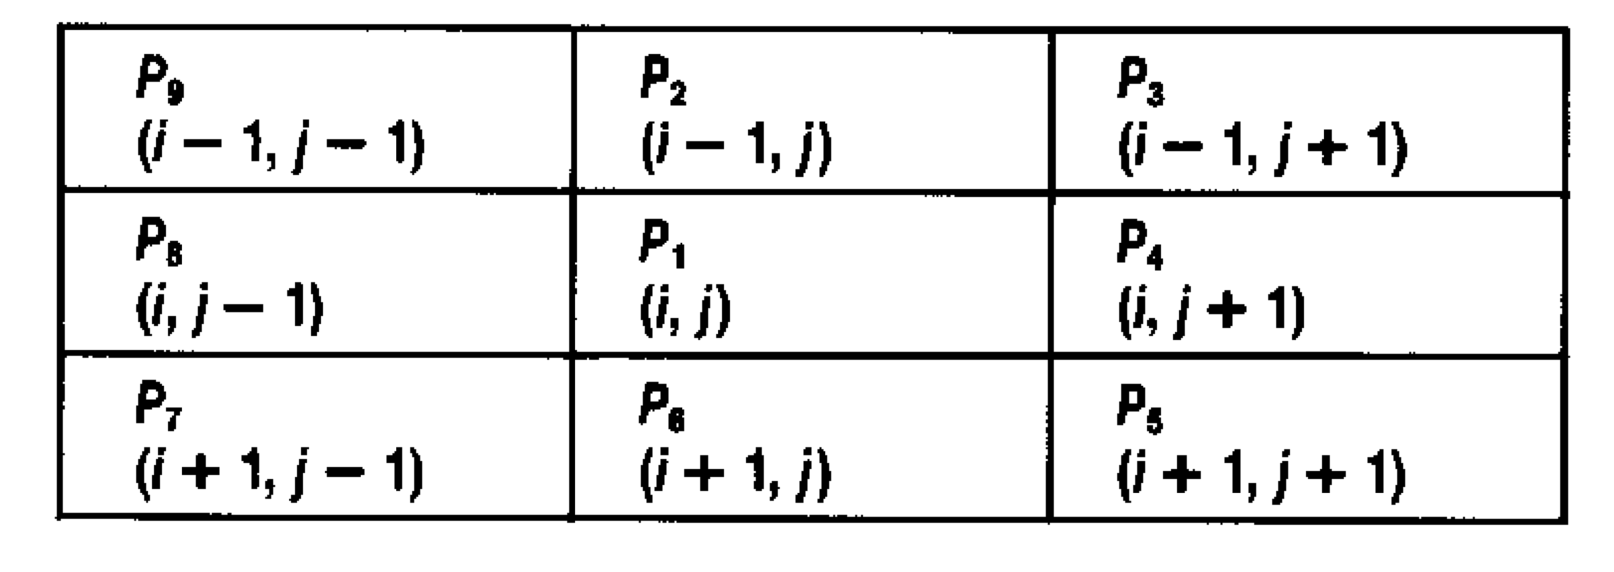
\includegraphics[width=8cm]{Res/PixelNachbarschaft.png}


Der Algorithmus entfernt alle Randpunkte des Musters, außer den Pixeln welche Bestandteil des Skeletts sind. Um die Verbundenheit des Skeletts zu gewährleisten wird ein  Iterationsschritt in zwei Subiterationen aufgeteilt.

In der ersten Subiteration wird der Punkt P1 aus dem Muster gelöscht wenn er folgende Bedingungen erfüllt:\\ \\
a)2<=B(P1)<=6     
Bà Anzahl der Nachbarn von P1 !=0
Die Anzahl der Nachbarn von P1 welche den Wert 1 haben, muss somit zwischen 2 und 6 liegen.\\ \\
b) A(P1)=1
AàAnzahl der „01“-Folgen 
Die Anzahl der 01 Folgen in der geordneten Folge P2,P3...P9 muss genau eins betragen.\\ \\
c) P2*P4*P6=0  
Mindestens ein Pixel der Pixelmenge P2, P4, P6 muss den Wert Null haben.\\ \\
d) P4*P6*P8=0
Mindestens ein Pixel der Pixelmenge P4, P6, P8 muss den Wert Null haben.
\\

Sind alle Bedingungen a, b ,c und d erfüllt so wird der Wert des Pixels auf 0 gesetzt.
Dies bedeutet dass er kein Teil des Skelett-Musters mehr ist.
Wird eine der Bedingungen nicht erfüllt, so bleibt der Pixelwert bei 1.\\

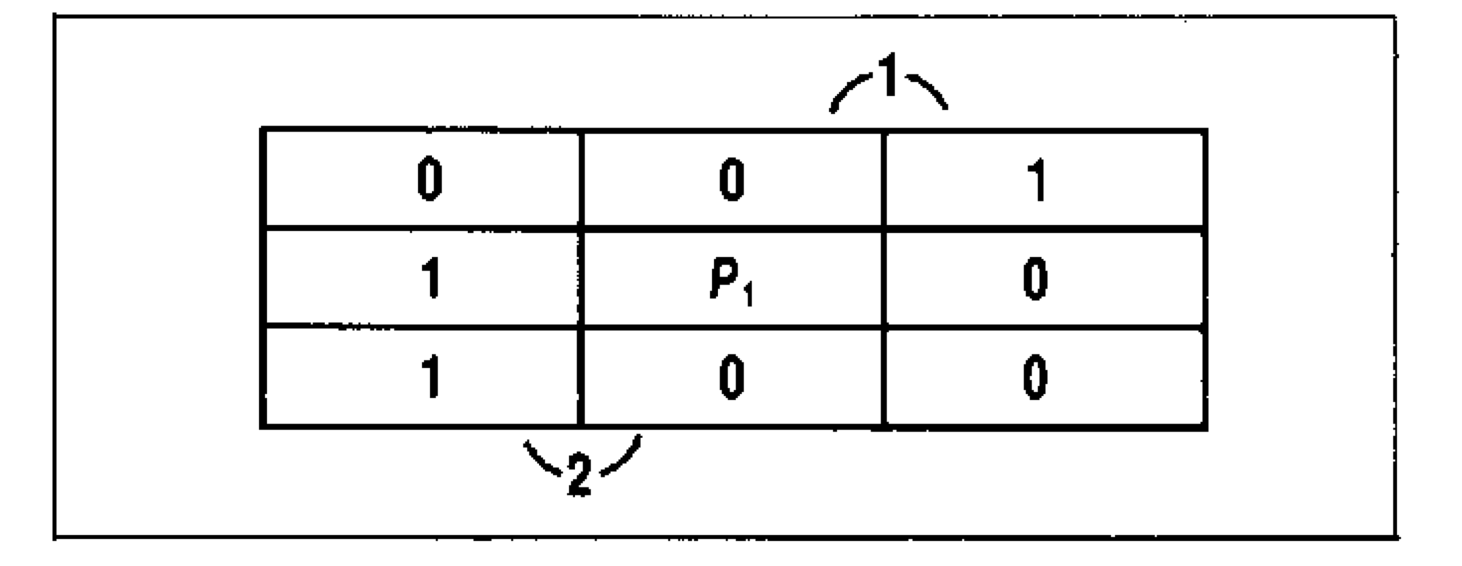
\includegraphics[width=8cm]{Res/01Folgen.png}


In der zweiten Subiteration wird P1 gelöscht falls folgende Bedingungen gelten: \\ \\
a) 2<=B(P1)<=6 \\ \\
b) A(P1)=1 \\ \\
c) P2*P4*P8=0 \\ \\
d) P2*P6*P8=0 \\ \\
In der zweiten Subiteration haben sich nur die Bedingungen c und d geändert.\\

Um die Bedingungen der ersten Subiteration zu erfüllen muss
P4=0 oder P6=0 oder (P2=0 und P8=0)  erfüllt sein.
Dies impliziert dass P1 entweder Süd- oder Ost-Grenzpunkt, oder Nordwesteckpunkt ist.
Um die Bedingungen der zweiten Subiteration zu erfüllen muss
P2=0 oder P8=0 oder (P4=0 und P6=0) sein.
Das heißt P1 ist Nord -oder West-Grenzpunkt oder Südosteckpunkt ist.

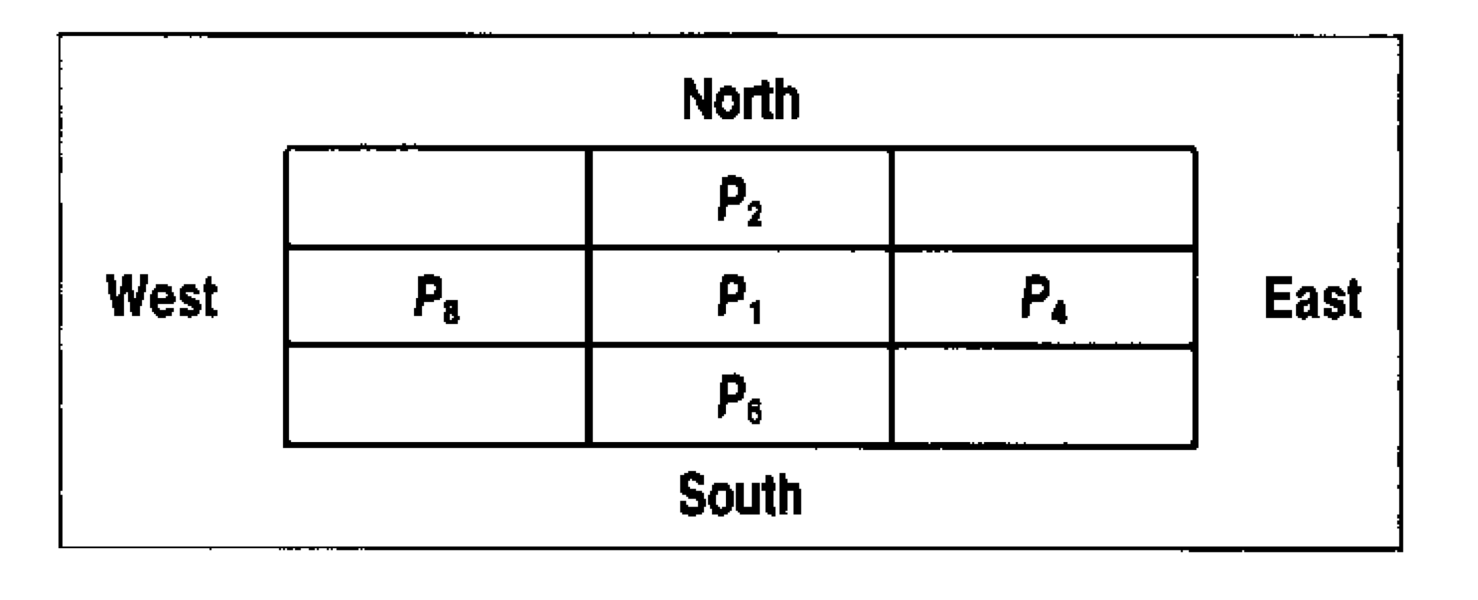
\includegraphics[width=8cm]{Res/Orientierung.png}


Während mit Bedingung a (2<=B(P1)<=6) die Endpunkte des Skeletts erhalten werden, so wird mit Bedingung b (A(P1)=1) die Auslöschung von Punkten zwischen den Endpunkten der Skelettlinie verhindert.\\

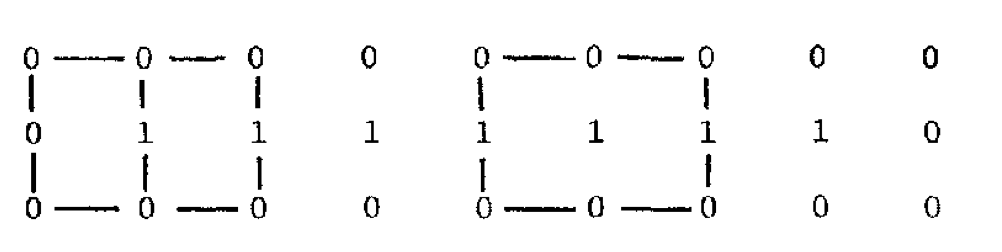
\includegraphics[width=8cm]{Res/EndpktVerbheit.png}

In der Matrix Search M befinden sich während der ersten Iteration alle Pixel die gelöscht werden dürfen, da sie den Bedingungen der ersten Iteration genügen. Ist dies nicht der Fall, so ist der Counter=0 und der Algorithmus beendet, da es anscheinend keine zu löschenden Pixel mehr gibt. Die Skelettierung ist somit beendet.
Falls der Counter ungleich null ist, werden die Pixel welche den Bedingungen genügen von der Matrix IT (Skelett-Muster) abgezogen, der Counter wird null gesetzt und es wird zur zweiten Iteration fortgeschritten. Dort findet der Ablauf mit veränderten Bedinungen c und d nochmals statt. Ist auch nach dem Durchlaufen der zweiten Subitertation der Counter ungleich null so wird der Vorgang iterativ fortgeführt.\\




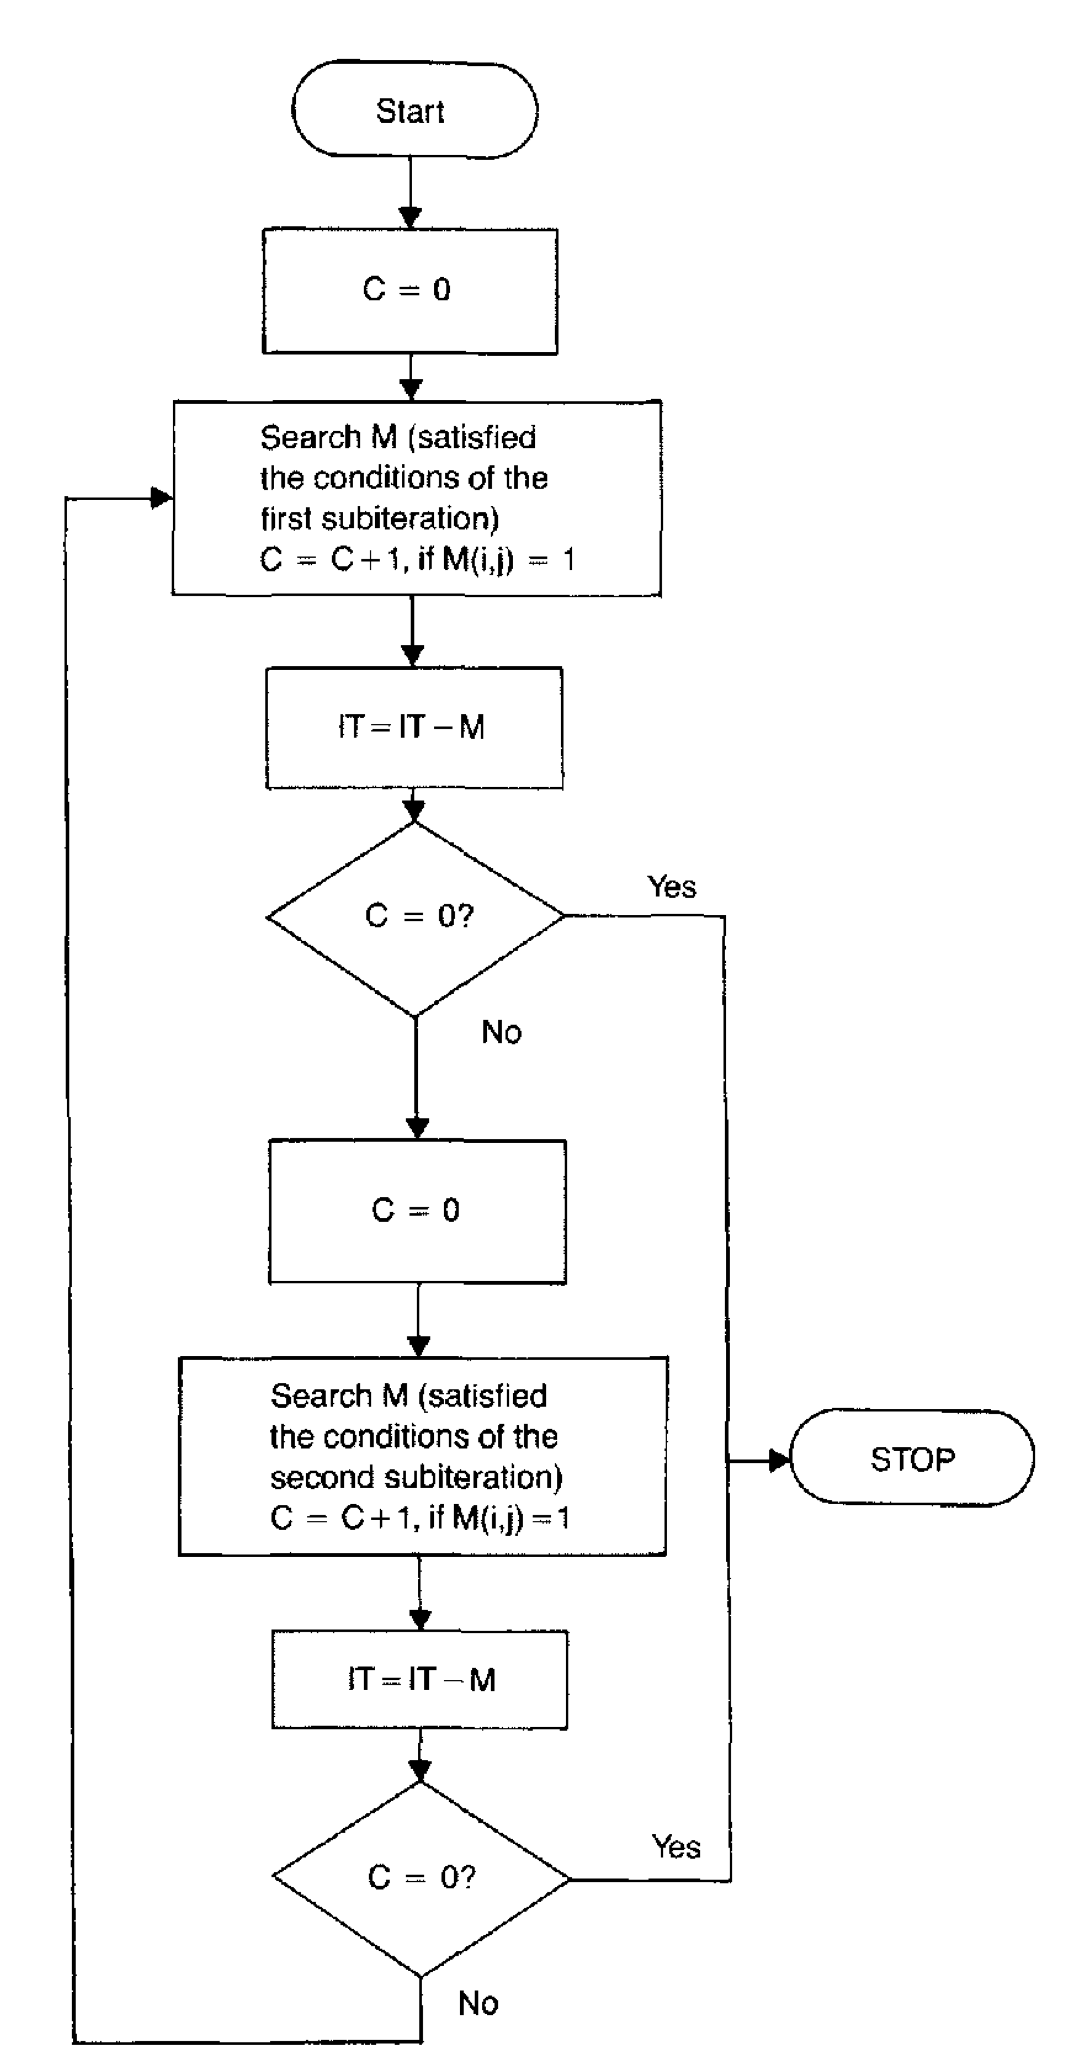
\includegraphics[width=6cm]{Res/AlgUebersicht.png}


Der Algorithmus erzielt sehr gute Ergebnisse im Bezug auf Verbundenheit, und Rauschsicherheit bei Randpunkten. Die Bedingungen welche zum Auffinden der zu löschenden Randpunkte führen sind sehr simpel. Durch den Bezug auf die n-1te Iteration zur Abfrage der Bedingungen kann der Algorithmus sehr schnell ausgeführt werden, da keine Warteabhängikeiten bestehen.
